\chapter{Der Transformationssatz}
  \begin{definition}
    Eine Abbildung $\Phi: \script{U} \to \script{V} \ ,\script{U}, \script{V} \subseteq \mathbb{R}^n$ offen, heißt $C^1$-Diffeomorphismus, falls $\Phi$ bijektiv ist und $\Phi, \Phi^{-1}$ stetig differenzierbar sind.
  \end{definition}

  \begin{example}[Polarkoordinaten in $\mathbb{R}^n$]
    $\Phi: (0, \infty) \times (0, 2\pi) = \script{U} \to \script{V} = \mathbb{R}^2 \setminus \{(x,0) \ | \ x \geq 0\}$\\
    \\
    $\Phi(r, \script{C}) = (r \cos(\script{C}), r \sin(\script{C}))$\\
    $\Phi^{-1}(x,y) = \begin{cases}
      (r, \arccos(\frac{x}{r})) & \text{, falls } y \geq 0\\
      (r, 2\pi - \arccos(\frac{x}{r})) & \text{, falls } y < 0
    \end{cases}\\
    r = \sqrt{x^2 + y^2}$\\
    \\
    Für $x < 0$ filt alternativ $\Phi^{-1}(x,y) = (r, \frac{\pi}{2} + \arccos(\frac{x}{r}))\\
    \implies \Phi^{-1}$ glatt auf ganz $\script{V} \implies \Phi^{C^1}$ Diffeomorphismus.
    \begin{center}
      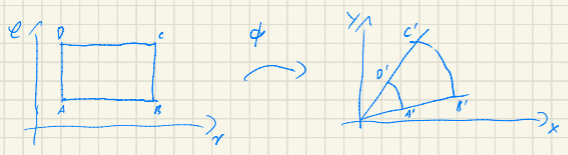
\includegraphics[height=2cm]{img/VII_Bsp_1_Polarkoordinaten.png}
    \end{center}
  \end{example}

  \begin{remark}[Notation]
    $x \in \mathbb{R}^n, \delta >0$\\
    $Q(x, \delta) = \{y \in \mathbb{R}^n \ | \ ||y-x||_{\infty} \leq \delta\}, ||x||_{\infty} = \max\limits_{1 \leq k \leq n} | x_k |$
    \begin{center}
      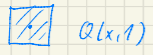
\includegraphics[height=1cm]{img/VII_Notation_1_Qx1.png}
    \end{center}
  \end{remark}

  \begin{lemma}
    Sei $\script{U} \subseteq \mathbb{R}^n$ offen, $x_0 \in \script{U}$ und $\Phi: \script{U} \to \mathbb{R}^n$ mit $D\Phi(x_0) \in GL_n(\mathbb{R})$. Gegeben sei eine Folte $Q_j = Q(x_j, \phi_j)\subseteq \script{U}$ mit $\phi_j \to 0$ und $x_0 \in Q_j \ \forall \ j \in \mathbb{N}$. Dann gilt:
    $$\limsup\limits_{j \to \infty} \frac{\lambda^n(\Phi(Q_j))}{\lambda^n(Q_j)} \leq |det D\Phi(x_0)|$$
  \end{lemma}
  \begin{proof}
    siehe Aufschrieb
  \end{proof}

  \begin{theorem}[Transformationsformel]
    $\script{U}, \script{V} \subseteq\mathbb{R}^n$ offen, $\Phi:\script{U} \to \script{V} C^1$-Diffeomorphismus. Ist $A \subseteq \script{U}$ $\lambda^n$-messbar, so ist auch $\Phi(A)$ $\lambda^n$-messbar und es gilt:
    \begin{enumerate}
      \item $\lambda^n(\Phi(A)) = \int\limits_A | \det D\Phi(x) | dx$
    \end{enumerate}
    Weiter gilt für jede $\lambda^n$-messbare Funktion $f: \script{V} \to \bar{\mathbb{R}}$:
    \begin{enumerate}[resume]
      \item $\int\limits_{\script{V}} f(y) dy = \int\limits_{\script{U}} f(\Phi(x)) |\det D\Phi(x)| dx \ \ (dy \ \hat{=} \ d\lambda^n(y))$
    \end{enumerate}
    falls eines der Integrale definiert ist.
  \end{theorem}

  \begin{proof}
    siehe Aufschrieb
  \end{proof}

  \sidenote{Vorlesung 20}{22.01.2021}
  \begin{example}
    \begin{enumerate}
      \item[]
      \item
        \begin{align*}
          f:\mathbb{R}^2 \to \mathbb{R}, f(x,y) = e^{-(x^2+y^2)} = e^{-||(x,y)||^2}\\
          \int\limits_{\mathbb{R}^2} f d\lambda^2 \stackrel{\text{Fubini}}{=} \int\limits_{\mathbb{R}} e^{-x^2}(\int\limits_{\mathbb{R}} e^{-y^2} dy) dx = (\int\limits_{\mathbb{R}}^{-x^2} dx)^2
        \end{align*}
        Für Polarkoordinaten $\Phi:(0,\infty) \times (0,2\pi) \to \mathbb{R}^2 \setminus \{(x,0) \ | \ x \geq 0\}$ gilt: \\
        $$\det D\Phi(r,\Theta) = r$$\\
        Da $\{(x,0) \ | \ x \geq 0\}$ eine $\lambda^2$-Nullmenge ist, folgt aus der Transformationsformel:
        \begin{align*}
          \int\limits_{\mathbb{R}^2} f d\lambda^2
          &= \int\limits_{(0,\infty) \times (0,2\pi)} e^{-r^2} d\lambda^2(r,\Theta)\\
          &\stackrel{\text{Fubini}}{=} \int\limits_0^{\infty} e^{-r^2}r(\int\limits_0^{2\pi}d\Theta)dr\\
          &= 2\pi \int\limits_0^{\infty} e^{-r^2} r dr\\
          &= 2\pi [-\frac{1}{2} e^{-r^2}]_{r=0}^{r=\infty}\\
          &= \pi\\
          \implies \int\limits_0^{\infty} e^{-x^2} dx &= \sqrt{x}
        \end{align*}
      \item Spezialfall $\Phi: \script{U} \to \script{V} C^1$-Diffeomorphismus ist Einschränkung einer linearen Abbildung.
        \begin{align*}
          &\implies \Phi(x) = Sx \text{ mit } S\in GL_n(\mathbb{R})\\
          &\implies D\Phi(x) = S \ \forall \ x \in \script{U}\\
          &\stackrel{Trafo}{\implies} \lambda^n(S(D)) = |\det S| \lambda^n(D) \text{ (siehe Satz ???)}\\
          \text{bzw. } \int\limits_{\script{V}} f(y) d\lambda^n(y) &= |\det S| \int\limits_{\script{U}} f(Sx) d\lambda^n(x)
        \end{align*}
      \item Polarkoordinaten im $\mathbb{R}^3$\\
        $$\Phi(r, \Theta, \phi) = (r \sin(\Theta) \cos(\phi), r \sin(\Theta)\sin(\phi), r \cos(\Theta))$$ ist $C^{\infty}$-Diffeomorphismus der offenen Mengen $\script{U} = (0,\infty) \times (0,\pi) \times (0,2\pi)$ und $\script{V} = \mathbb{R}^3 \setminus \{(x,0,z) \ | \ x \geq 0\}$\\
        Inverse:\\
        $r=\sqrt{x^2 + y^2 + z^2}, \Theta = \arccos(\frac{z}{r})$\\
        $\phi = \begin{cases}
          \arccos(\frac{x}{\sqrt{x^2 + y^2}}) & \text{, für } y \geq 0\\
          2\pi - \arccos(\frac{x}{\sqrt{x^2 + y^2}}) & \text{, für } y \leq 0
        \end{cases}$\\
        $D\Phi(r, \Theta, \phi) = \left(\begin{array}{ccc}
          \sin(\Theta)\cos(\phi) & r\cos(\Theta)\cos(\phi) & -r\sin(\Theta)\sin(\phi)\\
          \sin(\Theta)\sin(\phi) & r\cos(\Theta)\sin(\phi) & r\sin(\Theta)\cos(\phi)\\
          \cos(\Theta) & -r\sin(\Theta) & 0
        \end{array} \right)$
        \begin{align*}
          &\implies \det D\Phi = r^2 \sin(\Theta)\\
          E &:= [r_1, r_2] \times [\Theta_1, \Theta_2] \times [\phi_1, \phi_2]\\
          \lambda^3(\Phi(E)) &= \int\limits_{r1}^{r2}\int\limits_{\Theta_1}^{\Theta_2}\int\limits_{\phi_1}^{\phi_2} r^2 \sin(\Theta) d\phi d\Theta dr = \frac{r_2^3 - r_1^3}{3} (\cos(\Theta_1) - \cos(\Theta_2)) (\phi_2 - \phi_1)
        \end{align*}
    \end{enumerate}
  \end{example}

  \begin{remark}
    \underline{Ziel:} Umrechnung von Differentialoperatoren\\
    Begriff: $\Phi: \script{U} \to \script{V} C^k$-Diffeomorphismus zwischen $\script{U}, \script{V}$ offen.\\
    Gramsche Matrix $g \in C^{k-1}(\script{U}, \mathbb{R}^{n\times n}), g = (g_{i,j})$
    $$g(x) = D\Phi(x)^{\top} D\Phi(x) \text{ bzw.}\\
    g_{i,j}(x) = <\frac{\partial\Phi}{\partial x_i}(x), \frac{\partial\Phi}{\partial x_j}(x)>$$\\
    Für Polarkoordinaten im $\mathbb{R}^3$ gilt:
    $$(g_{i,j}(r, \Theta, \phi))_{1\leq i,j \leq 3} = \left(\begin{array}{ccc}
      1 & 0 & 0 \\
      0 & r^2 & 0 \\
      0 & 0 & r^2 \sin^2(\Theta)      
    \end{array}\right)$$
    
    \newpage

    Allgemein gilt:\\
    $g(x)$ ist symmetrisch und strikt positiv definit, denn
    $$<g(x)v,v> \ = \ <D\Phi(x)^{\top}D\Phi(x) v, v> \ = |D\Phi(x) v|^2 > 0$$
    für $v\neq 0$ und $D\Phi(x) \in GL_n(\mathbb{R}) \implies g(x)$ ist invertierbar.\\
    \\
    Wir setzen: $g^{ij}(x) = (g(x)^{-1})_{ij}$\\
    ... (Rest siehe Aufschrieb)
  \end{remark}

  \begin{theorem}
    Sei $\Phi \in C^1(\script{U}, \script{V})$ Diffeomorphismus zwischen $\script{U}, \script{V} \subseteq \mathbb{R}^n$ offen mit gramscher Matrix $(g_{ij})$
    \begin{enumerate}
      \item Für $v \in C^1(\script{V})$ gilt mit $\mu = v \circ \Phi$:
      $$(\triangledown v) \circ \Phi = D\Phi \cdot \triangledown_g u \ \ , \ \ \triangledown_g u := \sum\limits_{i,j=1}^n g^{ij} \frac{\partial u}{\partial x_i} e_j$$
      \item Für $y \in C^1(\script{V}, \mathbb{R}^n)$ gilt mit $y \circ \Phi = D\Phi x$:
        $$(div(y)) \circ \Phi = div_g x := \frac{1}{\sqrt{det(g)}} \sum\limits_{j=1}^n \frac{\partial}{\partial x_j} (\sqrt{det(g)} x_j)$$
      \item Ist $\Phi \in C^2(\script{U}, \script{V}), v \in C^2(\script{V}), u = v \circ \Phi$
        $$\implies (\triangle v) \circ \Phi = div_g \triangledown_g u = \frac{1}{\sqrt{det(g)}} \sum\limits_{i,j=1}^n \frac{\partial}{\partial x_i} (\sqrt{det(g)} g^{ij} \frac{\partial u}{\partial x_j})$$
    \end{enumerate}
  \end{theorem}
  \begin{proof}
    siehe Aufschrieb
  \end{proof}

  \begin{example}[Laplace in Polarkoordinaten im $\mathbb{R}^3$]
    \begin{align*}
      \triangledown_g u &= \frac{\partial u}{\partial r} e^r + \frac{1}{r^2} \frac{\partial u}{\partial \Theta} e^{\Theta} + \frac{1}{r^2 \sin^2(\Theta)} \frac{\partial u}{\partial \phi} e^{\phi}\\
      div_g x &= \frac{1}{r^2} \frac{\partial}{\partial r} (r^2 x^r) + \frac{1}{\sin(\Theta)} \frac{\partial}{\partial \Theta} (\sin(\Theta) x^{\Theta}) + \frac{\partial x^{\phi}}{\partial \phi}\\
      \triangle_g u &= \frac{1}{r^2} \frac{\partial}{\partial r} (r^2 \frac{\partial u}{\partial r})  + \frac{1}{r^2 \sin(\Theta)} \frac{\partial}{\partial \Theta} (\sin(\Theta) \frac{\partial u}{\partial \Theta}) + \frac{1}{r^2 \sin^2(\Theta)} \frac{\partial^2 u}{\partial \phi^2}
    \end{align*}
    $e^r, e^{\Theta}, e^{\phi}$ Standardbasis im $(r, \Theta, \phi)$-Raum und $x^r, x^{\Theta}, x^{\phi}$ sind zugehörige Koordinaten
    $$v(x,y,z) = (x^2 + y^2 + z^2)^{-\frac{1}{2}} \implies u = r^{-1}$$
    $$\implies \triangle v\circ \Phi = \triangle_g u = 0 \text{ auf }\mathbb{R}^3\setminus\{0\}$$
  \end{example}